\chapter[Detection of Cosmic-rays]{\centering Detections of Cosmic-Rays \\}\label{Ch:CR_Detection}

\section{Extensive Air Showers}

Use Earth's atmosphere as an interaction medium.
Primary particle interacts with the molecules in the atmosphere to produce a cascade of secondary particles. This cascade of particles is referred to as an Extensive Air Shower (EAS).
Hadronic primaries can produce pions, muons and other stuff.
Mixture of a hadronic core with an electromagnetic component from the decay of $\pi^{0}$.

Shower profile has particles produced until energy on individual secondary particles drop below the ionization threshold. Therefore the shower will reach a point of maximum particle number then will drop off.

\begin{figure}
\centering
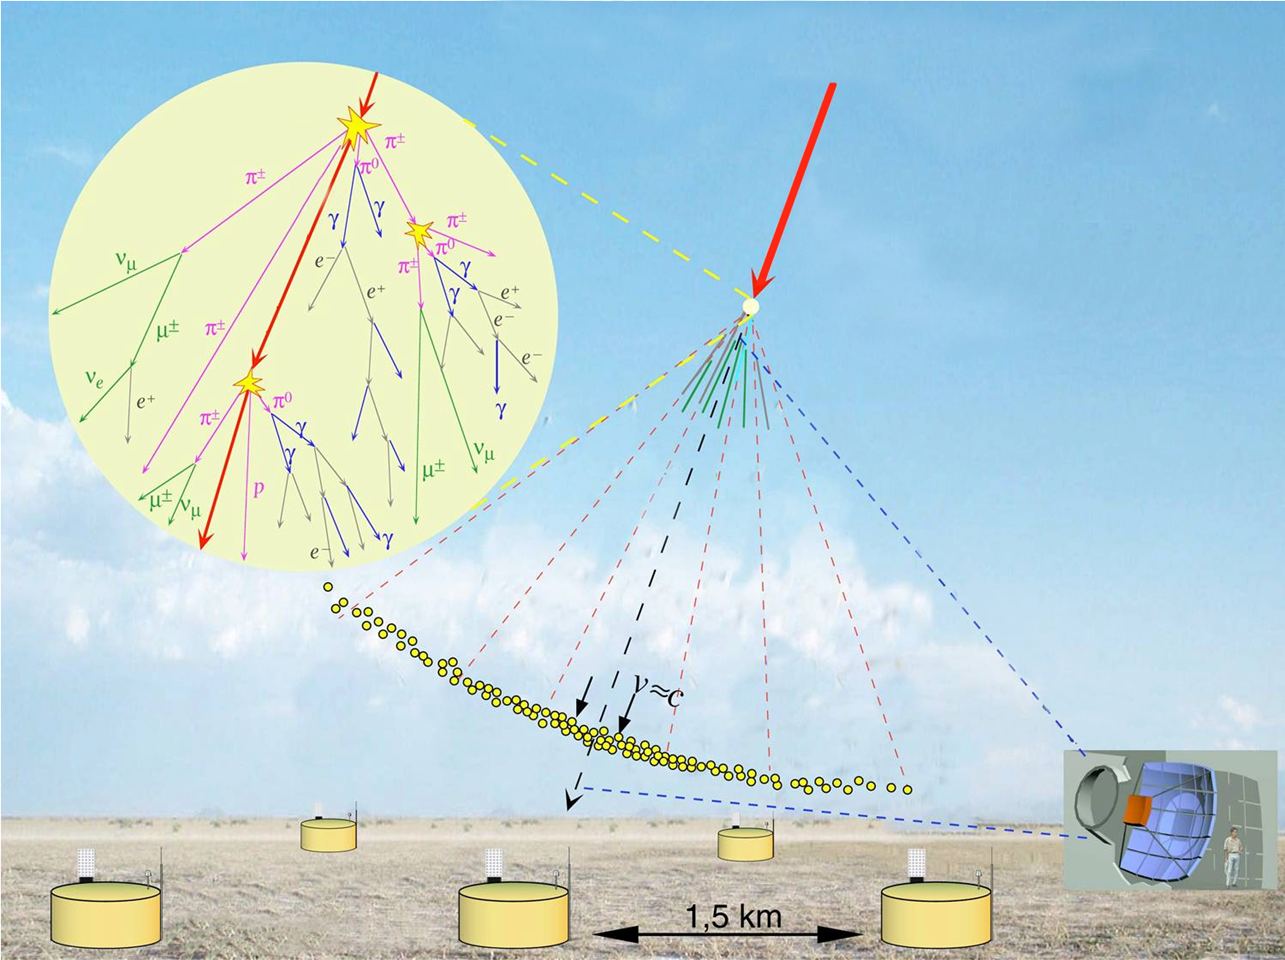
\includegraphics[width=0.7\textwidth]{chapters/pix/CR_ExtensiveAirShowers.png}
\caption{Diagram of Cosmic-ray Extensive Air Showers.}
\end{figure}

Above energies of 100 TeV (10$^{14}$ eV) direct detection becomes increasingly difficult \cite{RevModPhys.71.S165}. Ground based observations are made by exploiting extensive air showers (EAS). EAS were first discovered by Pierre Auger in 1932 when noticed that cosmic-rays were arriving at different detectors at the same time. He formed the conclusion that they were secondary particles emitted from the same source \cite{RevModPhys.11.288}.

An extensive air shower is a cascade of secondary particles that begins when the cosmic ray
first interacts with the earth’s atmosphere. Three main components of an extensive air shower are:

\begin{itemize}
\item Electromagnetic - consisting of electrons, positrons and $\gamma$-rays resulting from the decay of charged and neutral pions and kaons.
\item Hadronic component - consisting of heavy nuclei, charged pions and kaons.
\item Muonic - consisting of muons and neutrinos resulting from the decay of charged pions and kaons.
\end{itemize}

The height at which cosmic rays interact within the atmosphere is dependent on their energy and composition. A measure of the amount of atmospheric matter above ground level is called the atmospheric or slant depth $X$. The unit of slant depth is usually g/cm$^2$. To calculate the slant depth, firstly need to define a vertical atmospheric depth.
\begin{equation}
X_v = \int^{\infty}_{h} \rho(h') dh'
\end{equation}
where $X_v$ is the vertical atmospheric depth and $\rho$ is the atmospheric density. Now a slant depth can be defined.  
\begin{equation}
X = \frac{X_v}{\mathrm{cos}(\theta)}
\end{equation}
where $\theta$ is the angle from the zenith. Shower age $s$ is a parameter often used to describe the development of an extensive air shower relative to shower maximum. The slant depth at which shower maximum occurs is defined as depth of maximum development ($X_{max}$). Shower age is defined as
\begin{equation}
s(X) = \frac{3}{(1 + 2 X_{max} / X)}
\end{equation}

\section{Electromagnetic Component}

\begin{figure}[htp]
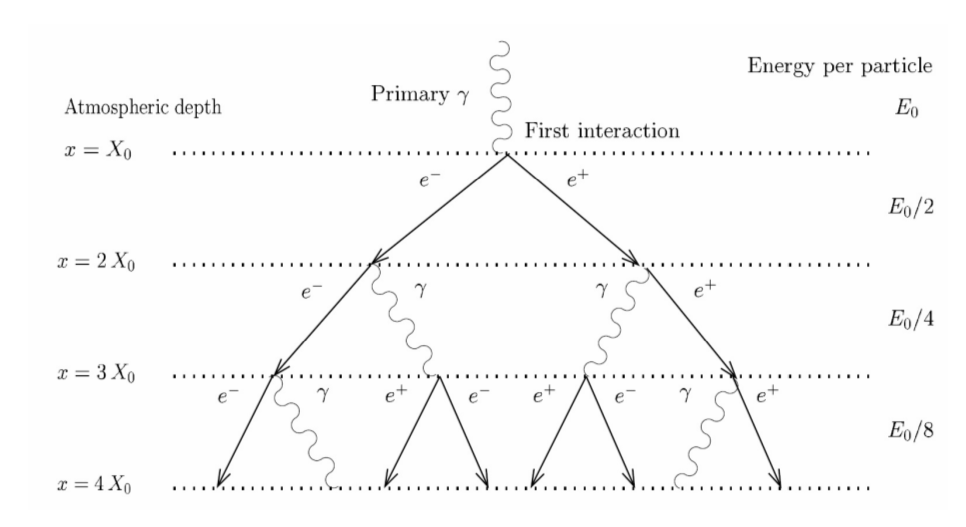
\includegraphics[width=\textwidth]{chapters/pictures/heilter_model_EM.png}
\caption{A graphical representation of the Heitler model.}\label{fig:heitler_model}
\end{figure}

To describe the electromagnetic shower, a simple model was proposed by Heitler \cite{Heitler}. In this model a $\gamma$-ray of $E_0$ interacts with an atmospheric nucleus (N), creating an electron-positron pair via pair-production
\begin{equation}
\gamma + N \rightarrow e^+ + e^- 
\end{equation}
Each of the electron and positron then give half of their energy to $\gamma$-ray via bremsstrahlung
\begin{equation}
e^{\pm} + N \rightarrow N + e^{\pm} + \gamma
\end{equation}
This process continues as shown in Figure \ref{fig:heitler_model} until the energy of the particles falls below the critical energy $E_C$ required for further particle production, and ionisation begins to dominate.

The energy of each shower particle after $n$ radiation lengths will be
\begin{equation}
E(n) = \frac{E_0}{2^n}
\end{equation}

Once the individual particles energy drops below the energy where ionisation dominates no more particles are produced. Therefore the maximum particle number is
\begin{equation}
N_{max} = \frac{E_0}{E_C}
\end{equation}

\section{Hadronic Component}

\begin{figure}[htbp]
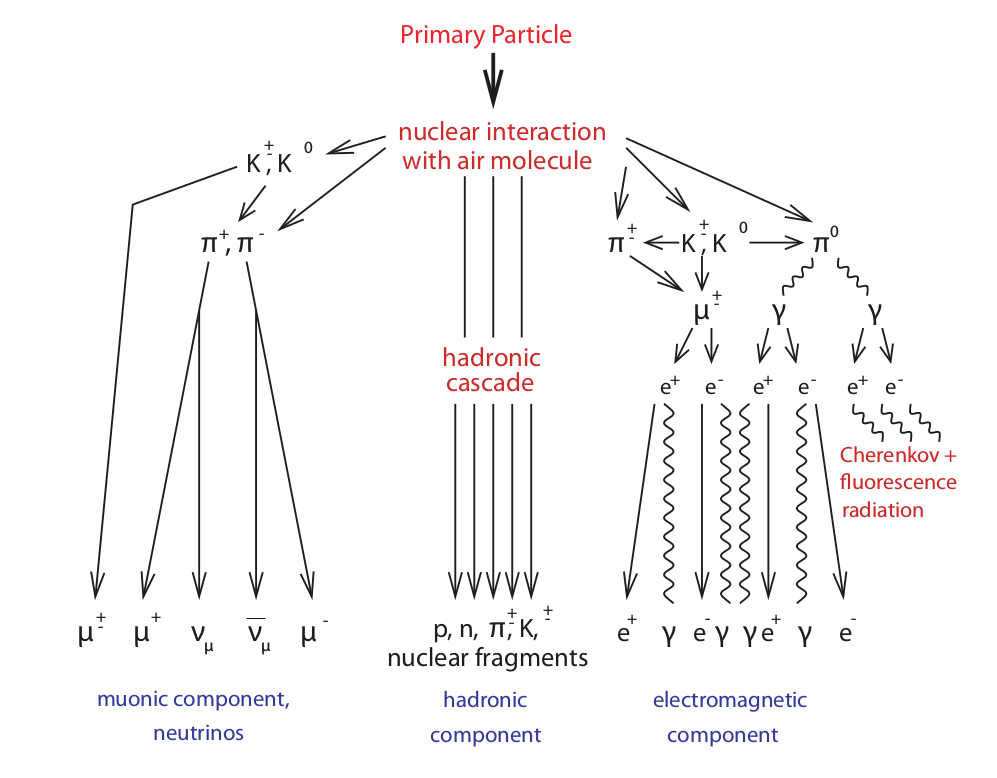
\includegraphics[width=\textwidth]{chapters/pictures/hielter_model_hadronic.png}
\caption{A graphical representation of the Heitler model for an extensive air shower initiated by a hadronic primary. Image taken from \cite{0034-4885-66-7-202}.}
\end{figure}

A hadronic EAS is initiated the same way in the atmosphere as a electromagnetic shower but the interaction produces kaons and charged and neutral pions \cite{kumpel}. An approach similar to Heitler's treatment of electromagnetic cascades can be used to explain the basic properties of hadronic cascades. The atmospheric is divided into layers, with the thickness of each layer characterised by an interaction length $\lambda_I$. After travelling one interaction length, the primary hadron interacts with the atmosphere and produces $2N$ charged pions and $N$ neutral pions. The neutral pions decay into two photons
\begin{equation}
\pi^0 \rightarrow \gamma + \gamma
\end{equation}
These photons can initiate electromagnetic cascades, and the charged pions becoming the next generation of the hadronic shower. The process continues until the energy of the pions drops below a critical energy $E^I_{crit} \approx$ 20 GeV. The critical energy is the point where the decay length becomes shorter than the interaction length. At this threshold, the charged pions decay
\begin{eqnarray}
\pi^+ & \rightarrow & \mu^+ + \nu_{\mu} \\
\pi^- & \rightarrow & \mu^- + \bar{\nu}_{\mu}
\end{eqnarray}

\section{Fluorescence Production}

The charge particles of EAS interact with the nitrogen molecules in the atmosphere. This interaction turns the nitrogen molecule dipole like and when the nitrogen returns to a ground state, a photon is emitted. This emitted photon is termed fluorescence light. Fluorescence light is can be emitted isotropically and typically in the UV band (between 300 and 400 nm). *** Show wavelength profile ***


\section{Atmospheric Effects}




\section{Detectors and History}

%Early Experiments:
%
%Volcano Ranch
%
%Haverah Park
%
%SUGAR
%
%Yakutsk array is located in Russia and has been operating in different forms since 1967. The array reached a maximum collecting area of 17 km$^2$ around 1990. Recently it has been reconfigured to have a collection area of 8 km$^2$ to study lower energy cosmic-rays.
%
%Akeno Gaint Air Shower Array (AGASA) is located in Tokyo, Japan. Operating at an average altitude of 667 m above sea level from 1990 to 2004. The array consist of over one hundred scintillator detectors covering 100 km$^2$ ***check this***. The timing measurements and data collection is achieved via interconnected optical fibers.
%
%The Fly's Eye was the first successful air fluorescence detector operating from 1981 to 1993 at the Dugway Proving Grounds in Utah, USA. Fly's Eye achieved a time averaged aperture of about 100 km$^2$sr at the highest energies, considering it only operated on clear moonless nights. 
%
%HiRes improved on the Fly's Eye design by advancing resolution and sensitivity, This was achieved by increasing the telescope effective mirror area to 3.8 m$^2$ and reducing the camera pixel angular diameter to 1\textdegree. 

\textbf{Volcano Ranch 1959 until 1963.} First giant air shower array, located near Albuquerque, New Mexico. The array consisted of nineteen detectors located on a triangular gird, with an additional 20$^{\text{th}}$ detector being used in several different position throughout operation. For some of the operating period, the 20$^{\text{th}}$ detector was shielded by 10 cm of lead to investigate the penetrating (mounic) component of extensive air showers. Each detector was a 3.3 m$^2$ plastic scintillator viewed by a 5 inch photomultiplier tube. The array was operated in two configurations: first used with spacing of 442 m (covering 2 km$^2$) and later increased to a spacing of 884 m (covering 8 km$^2$). 

\noindent \textbf{Haverah Park 1968 until 1987.} A 12 km$^2$ ground array located at Haverah Park, England. This experiment used water Cherenkov tanks. The irregular design of the array was a consequence of limited land access which dictated the placement of detectors.
					
\noindent \textbf{SUGAR (Sydney University Giant Airshower Recorder) 1968 until 1979.} Located in the Pilliga State Forest, New South Wales, Australia. SUGAR was the first large detector to operate in the southern hemisphere (Pierre Auger Observatory being the second). At its peak operation, SUGAR consisted of 47 detectors situated over an area of approximately 70 km$^2$. The majority were located on a square grid of 1600 m spacing, with some detectors located on a smaller grid of either 800 or 400 m spacing to gather data on smaller showers. Each detector consisted of two liquid-scintillators separated by 50 m and buried approximately 1.5 m underground. 
					
\noindent \textbf{Yakutsk 1970 until present.} Located in Yakutsk, Russia. It has undergone many reconfigurations throughout the years. An expansion in 1974 achieved a collecting area of approximately 18 km$^2$, but it was down sized in 1995 to cover about 10 km$^2$. Yakutsk contains scintillation detectors and up-ward facing PMTs. The up-ward facing PMTs are unique to Yakutsk (in terms of giant air shower arrays), that are used to detect the atmospheric Cherenkov light produced by EAS, from which a calorimetric estimation of primary energy can be made.
					
\noindent \textbf{Fly's Eye (I and II) 1981 until 1992.} While not the first detector to use the air fluorescence technique, it was the first detector to successfully detect large quantities of events. The first of two Fly's Eye detectors was built at Dugway Proving Grounds, Utah, approximately 160 km from Salt Lake City. Fly's Eye I began taking data in 1981, with a second detector, Fly's Eye II, was built 3.3 km away from Fly's Eye I and began operation in 1986. Both detectors consisted of PMTs to detect the fluorescence light emitted by atmospheric nitrogen. 
					
\noindent \textbf{AGASA (Akeno Giant Air Shower Array) 1990 until 2004.} Prior to the construction of the Pierre Auger Observatory, AGASA was the largest air shower array in the world. It was located 120 km west of Tokyo, Japan. Originally divided into four separate branches, AGASA was unified in 1995 to operate as a single detector. Construction of the main array began in 1987, with the smaller arrays located at the site having been constructed earlier. Data collection started in 1990 and continued until January 2004. AGASA covered approximately 100 km$^2$ with 111 2.2 m$^2$ plastic scintillator detectors spaced approximately 1 km apart.
					
\noindent \textbf{HiRes (High Resolution Fly's Eye) 1997 until 2006.} The High Resolution Fly's Eye observatory (HiRes) was the successor to the Fly's Eye experiment. It was located in the same place as its predecessor at the Dugway Proving Grounds in Utah. Two detectors named HiRes I and II comprised the experiment and began operation in 1997 and 1999 respectively. The two site were separated by a distance of 12.6 km.